\documentclass[9pt, a4paper, twocolumn]{article}
\usepackage[margin=1.8cm]{geometry}
\usepackage[utf8]{inputenc}
\usepackage[T1]{fontenc}
\usepackage{hyperref}
\usepackage{graphicx}
\usepackage{xcolor}
\definecolor{temperiert}{HTML}{2ca02c}
\definecolor{pythagoreisch}{HTML}{ffbf00}
\definecolor{rein}{HTML}{1f77b4}
\definecolor{reinZwei}{HTML}{d62728}
\definecolor{mitteltoenig}{HTML}{7f7f7f}
\definecolor{tonnetzTeal}{HTML}{11b7ad}
\usepackage{caption}
\usepackage{geometry}
\usepackage{booktabs}
\usepackage{enumitem}
\usepackage{pgfplots}
\usepackage{amsmath}
\usepackage{hyperref}
\pgfplotsset{compat=1.18}
\usepackage{tikz}
\usetikzlibrary{arrows.meta,positioning,calc}
\usepackage[small, raggedright]{titlesec}
\frenchspacing

\title{Seminar Intonation -- Wintersemester 2025 (HMDK)}
\author{
  Albert Mañosa Sardà\\
  \url{https://github.com/albertms10/intonation_25ws}\\
  Prof. Michael Flade
}
\date{5. Februar 2026}

\begin{document}

\maketitle

Diese Arbeit analysiert und vergleicht fünf verschiedene Intonationssysteme anhand desselben harmonischen Verlaufs. Ziel ist es, sowohl die klanglichen Eigenschaften der einzelnen Systeme als auch ihre Auswirkungen auf die Wahrnehmung eines extremen Modulationsprozesses zu beschreiben und zu bewerten.


\section{Musikalisches Ausgangsbeispiel}

Untersucht wird ein vierstimmiger, stark modulierender Akkordabschnitt aus Max Regers \emph{Beiträge zur Modulationslehre}. Der letzte Modulationsversuch dieses Beispiels führt von \textbf{ais-Moll} nach \textbf{Ces-Dur} und überbrückt damit einen sehr großen Abstand von \textbf{17~Quinten}.

\begin{figure}[h]
\centering
\vspace{-2mm}
\includegraphics[width=1\linewidth]{docs/reger.png}
\caption{Max \textsc{Reger}: \emph{Beiträge zur Modulationslehre} \S100: von ais-Moll nach Ces-Dur (ces-Moll)}
\end{figure}

Diese extreme Distanz macht den Abschnitt besonders interessant für den Vergleich verschiedener Intonationssysteme, da sich ihre charakteristischen Intervalle und Akkordverhältnisse hier klar akustisch nachvollziehen lassen.

\subsection{Harmonischer Ablauf}

\begin{enumerate}[label=\arabic*., itemsep=0\baselineskip, topsep=0\baselineskip]
\item Tonika ais-Moll;
\item Akkord der neapolitanischen Sexte (dis fis h) von ais-Moll; Umdeutung dieses Sextakkordes (dis fis h) zur 1. Versetzung der Oberdominante (H-Dur) von E-Dur;
\item Tonika E-Dur; Umdeutung dieses E-Dur zur Oberdominante in a-Moll;
\item Tonika a-Moll;
\item Akkord der neapolitanischen Sexte (d f b) von a-Moll; Umdeutung dieses Sextakkordes (d f b) zur 1. Versetzung der Tonika B-Dur (in B-Dur);
\item Unterdominante (Es-Dur) von B-Dur;
\item Akkord der neapolitanischen Sexte (es ges ces) von B-Dur; Umdeutung dieses Sextakkordes (es ges ces) zur 1. Versetzung der Tonika Ces-Dur (in Ces-Dur);
\item Oberdominante Ges-Dur;
\item Tonika Ces-Dur (ces-Moll).
\end{enumerate}

\begin{figure}[h]
\centering
\vspace{-6mm}
$$
\renewcommand{\arraystretch}{1.4}%
\begin{array}{l}
[\mathrm{ais}^{\mathrm{I}},\ \mathrm{ais}^{\mathrm{IV}^{6\natural}_{\sharp}}\ (= \mathrm{E}^{\underline{\mathrm{V}}}),\ \mathrm{E}^{\mathrm{I}}\ (= \mathrm{a}^{\mathrm{V}^{\sharp}}),\ \mathrm{a}^{\mathrm{I}},\ \mid \\

\mathrm{a}^{\mathrm{IV}^{6\flat}}\ (= \mathrm{B}^{\underline{\mathrm{I}}}),\ \mathrm{B}^{\mathrm{IV}},\ \mathrm{B}^{\mathrm{IV}^{6\flat}_{\flat}}\ (= \mathrm{Ces}^{\mathrm{I}}), \\

\left\{\begin{array}{l}
(= \mathrm{Ces}^{\mathrm{V}}),\ \mid\ \mathrm{Ces}^{\mathrm{I}}]\\
(= \mathrm{ces}^{\mathrm{V}^{\flat}}),\ \mid\ \mathrm{ces}^{\mathrm{I}}]
\end{array}\right.
\end{array}
$$
\vspace{-4mm}
\caption{Max \textsc{Reger}: \emph{Beiträge zur Modulationslehre} \S100: Modulationsprozess}
\end{figure}

\section{Darstellung im Tonnetz}

Zur Visualisierung des Modulationsprozesses wird das \textbf{Eulersche Tonnetz} verwendet. Es ermöglicht eine anschauliche Darstellung der Beziehungen zwischen Akkorden und Tonarten und zeigt insbesondere die Bewegung entlang des Quintenzirkels.

\begin{figure}[h]
\centering
\resizebox{0.48\textwidth}{!}{%
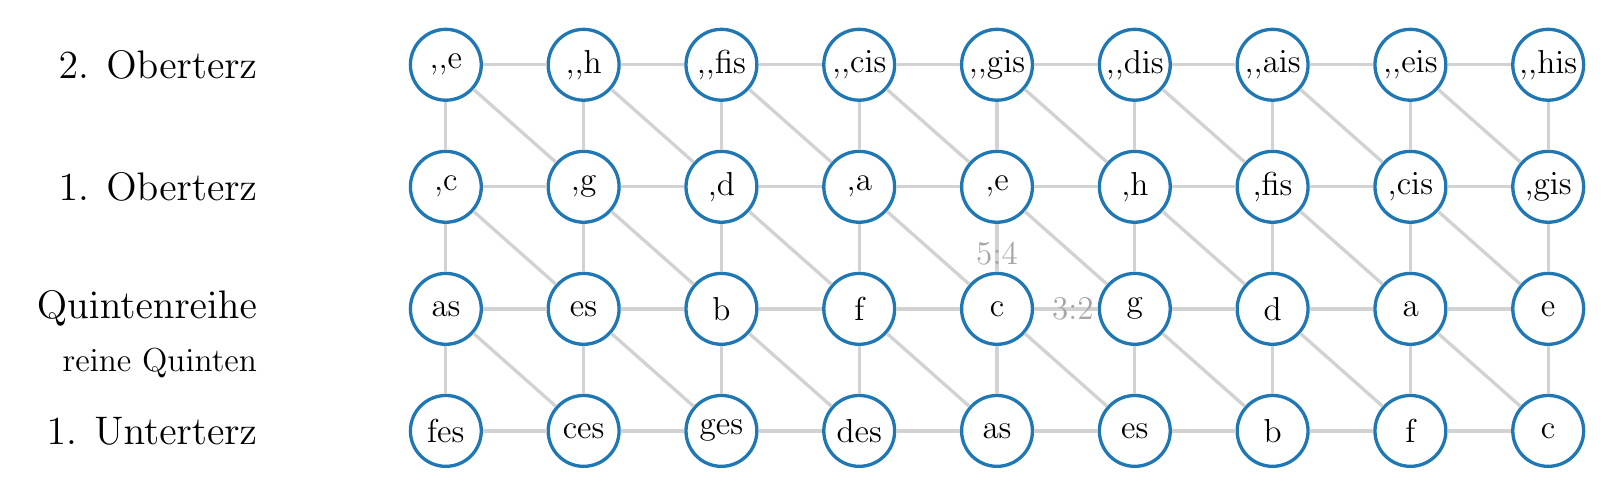
\begin{tikzpicture}[
  x=1.75cm,
  y=1.55cm,
  node/.style={circle, draw=rein, line width=1.2pt, minimum size=9mm, inner sep=0pt, font=\large},
  gridline/.style={gray!35, line width=1.2pt},
]

% Row labels
\node[anchor=east, font=\Large] at (-1.3,3) {2. Oberterz};
\node[anchor=east, font=\Large] at (-1.3,2) {1. Oberterz};
\node[anchor=east, font=\Large] at (-1.3,1) {Quintenreihe};
\node[anchor=east, font=\large] at (-1.3,0.55) {reine Quinten};
\node[anchor=east, font=\Large] at (-1.3,0) {1. Unterterz};

% Nodes (columns 0..8)
% y=3
\node[node] (t0) at (0,3) {,,e};
\node[node] (t1) at (1,3) {,,h};
\node[node] (t2) at (2,3) {,,fis};
\node[node] (t3) at (3,3) {,,cis};
\node[node] (t4) at (4,3) {,,gis};
\node[node] (t5) at (5,3) {,,dis};
\node[node] (t6) at (6,3) {,,ais};
\node[node] (t7) at (7,3) {,,eis};
\node[node] (t8) at (8,3) {,,his};

% y=2
\node[node] (u0) at (0,2) {,c};
\node[node] (u1) at (1,2) {,g};
\node[node] (u2) at (2,2) {,d};
\node[node] (u3) at (3,2) {,a};
\node[node] (u4) at (4,2) {,e};
\node[node] (u5) at (5,2) {,h};
\node[node] (u6) at (6,2) {,fis};
\node[node] (u7) at (7,2) {,cis};
\node[node] (u8) at (8,2) {,gis};

% y=1
\node[node] (v0) at (0,1) {as};
\node[node] (v1) at (1,1) {es};
\node[node] (v2) at (2,1) {b};
\node[node] (v3) at (3,1) {f};
\node[node] (v4) at (4,1) {c};
\node[node] (v5) at (5,1) {g};
\node[node] (v6) at (6,1) {d};
\node[node] (v7) at (7,1) {a};
\node[node] (v8) at (8,1) {e};

% y=0
\node[node] (w0) at (0,0) {fes};
\node[node] (w1) at (1,0) {ces};
\node[node] (w2) at (2,0) {ges};
\node[node] (w3) at (3,0) {des};
\node[node] (w4) at (4,0) {as};
\node[node] (w5) at (5,0) {es};
\node[node] (w6) at (6,0) {b};
\node[node] (w7) at (7,0) {f};
\node[node] (w8) at (8,0) {c};

% Grid lines: horizontals
\foreach \a/\b in {t0/t1,t1/t2,t2/t3,t3/t4,t4/t5,t5/t6,t6/t7,t7/t8,
                  u0/u1,u1/u2,u2/u3,u3/u4,u4/u5,u5/u6,u6/u7,u7/u8,
                  v0/v1,v1/v2,v2/v3,v3/v4,v4/v5,v5/v6,v6/v7,v7/v8,
                  w0/w1,w1/w2,w2/w3,w3/w4,w4/w5,w5/w6,w6/w7,w7/w8}
  \draw[gridline] (\a) -- (\b);

% Grid lines: verticals
\foreach \a/\b in {t0/u0,t1/u1,t2/u2,t3/u3,t4/u4,t5/u5,t6/u6,t7/u7,t8/u8,
                  u0/v0,u1/v1,u2/v2,u3/v3,u4/v4,u5/v5,u6/v6,u7/v7,u8/v8,
                  v0/w0,v1/w1,v2/w2,v3/w3,v4/w4,v5/w5,v6/w6,v7/w7,v8/w8}
  \draw[gridline] (\a) -- (\b);

% Grid lines: diagonals (down-right)
\foreach \a/\b in {t0/u1,t1/u2,t2/u3,t3/u4,t4/u5,t5/u6,t6/u7,t7/u8,
                  u0/v1,u1/v2,u2/v3,u3/v4,u4/v5,u5/v6,u6/v7,u7/v8,
                  v0/w1,v1/w2,v2/w3,v3/w4,v4/w5,v5/w6,v6/w7,v7/w8}
  \draw[gridline] (\a) -- (\b);

% Ratio labels (subtle, like in the reference image)
\node[gray!70, font=\large] at ($(u4)!0.55!(v4)$) {5:4};
\node[gray!70, font=\large] at ($(v4)!0.55!(v5)$) {3:2};

\end{tikzpicture}%
}
\caption{\href{https://de.wikipedia.org/wiki/Eulersches_Tonnetz}{Tonnetz}}
\end{figure}

Die Modulation führt von \textbf{ais-Moll} (10 Quinten über c) nach \textbf{Ces-Dur} (7 Quinten unter c), was insgesamt \textbf{17 absteigenden Quinten} entspricht. Reger wählt diese sehr entfernten Tonarten bewusst, um Doppelkreuz- oder Doppel-Bemoll-Töne zu vermeiden. Trotz der Länge des Weges bleibt der Prozess gut nachvollziehbar.

\begin{figure}[h]
\centering
\resizebox{0.3\textwidth}{!}{%
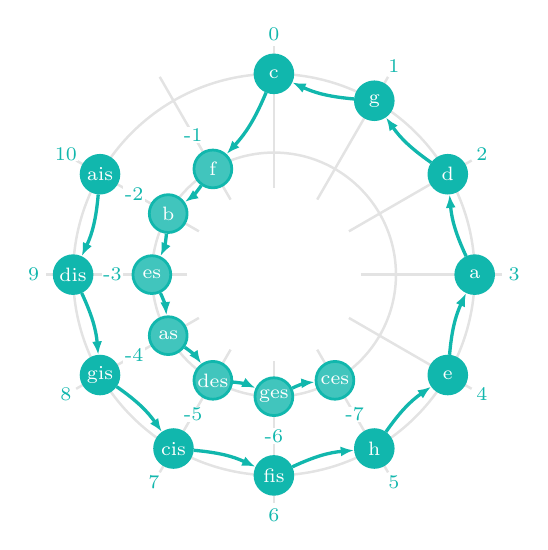
\begin{tikzpicture}[
  ring/.style={draw=gray!22, line width=0.9pt},
  spoke/.style={draw=gray!22, line width=0.9pt},
  nodeA/.style={circle, draw=tonnetzTeal, line width=1.0pt, fill=tonnetzTeal, text=white, minimum size=4.8mm, inner sep=0pt, font=\scriptsize},
  nodeB/.style={circle, draw=tonnetzTeal, line width=1.0pt, fill=tonnetzTeal!80, text=white, minimum size=4.8mm, inner sep=0pt, font=\scriptsize},
  path/.style={tonnetzTeal, line width=1.2pt, -{Latex[length=1.7mm]}},
  stepLabel/.style={font=\normalsize, text=tonnetzTeal, fill=white, inner sep=0.8pt},
]

\def\R{2.55} % outer radius
\def\r{1.55} % inner radius (more separation)

% two levels (enharmonic spellings share the same "circle section" / angle)
\draw[ring] (0,0) circle (\R);
\draw[ring] (0,0) circle (\r);

% 12 spokes
\foreach \k in {0,...,11} {
  \pgfmathsetmacro{\ang}{90-30*\k}
  \draw[spoke] (\ang:1.10) -- (\ang:2.90);
}

% Fifths index relative to c:
% c = 0; g = +1; ...; ais = +10; f = -1; ...; ces = -7.
%
% 17 descending fifths from ais (+10) to ces (-7):
% ais -> dis -> gis -> cis -> fis -> h -> e -> a -> d -> g -> c -> f -> b -> es -> as -> des -> ges -> ces
%
% Place nodes by fifths index (k) so that c is at the top (k=0).
% Level 1: k >= 0 (outer circle). Level 2: k < 0 (inner circle).
\foreach \i/\name/\k in {0/ais/10,1/dis/9,2/gis/8,3/cis/7,4/fis/6,5/h/5,6/e/4,7/a/3,8/d/2,9/g/1,10/c/0} {
  \pgfmathsetmacro{\ang}{90-30*mod(\k,12)}
  \node[nodeA] (n\i) at (\ang:\R) {\name};
  \node[font=\scriptsize, text=tonnetzTeal, fill=white, inner sep=0.2pt] at (\ang:\R+0.5) {\k};
}
\foreach \i/\name/\k in {11/f/-1,12/b/-2,13/es/-3,14/as/-4,15/des/-5,16/ges/-6,17/ces/-7} {
  \pgfmathsetmacro{\ang}{90-30*mod(\k,12)}
  \node[nodeB] (n\i) at (\ang:\r) {\name};
  \node[font=\scriptsize, text=tonnetzTeal, fill=white, inner sep=0.6pt] at (\ang:\r+0.5) {\k};
}

% spiral path (linear, step-by-step)
\foreach \i [evaluate=\i as \j using int(\i+1)] in {0,...,16} {
  \draw[path] (n\i) to[bend left=10] (n\j);
}

\end{tikzpicture}%
}
\caption{Quintenzirkel (Spirale, 2 Ebenen) -- 17 absteigende Quinten von ais nach ces.}
\end{figure}

Ein zentrales Mittel, das für viele Modulationen bei Reger charakteristisch ist, sind die \textbf{neapolitanischen Sextakkorde}, die schnelle Bewegungen im Quintenzirkel erlauben. Von den neun Akkorden der Modulation sind drei neapolitanische Sexten:

\vspace{-6mm}
\begin{align*}
\text{ais} &\to \text{h} \quad (-5\ \text{Quinten}) \\
\text{a} &\to \text{b} \quad (-5\ \text{Quinten}) \\
\text{es} &\to \text{ces} \quad (-4\ \text{Quinten})
\end{align*}
\vspace{-6mm}

\begin{figure}[h]
\centering
\resizebox{0.48\textwidth}{!}{%
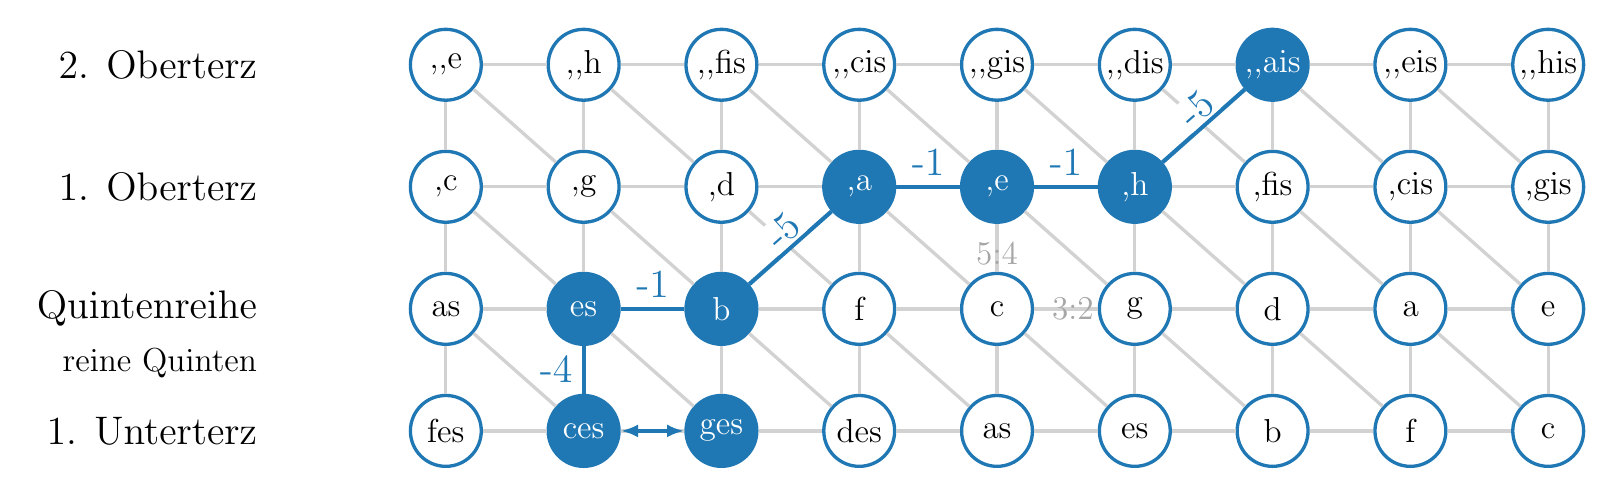
\begin{tikzpicture}[
  x=1.75cm,
  y=1.55cm,
  node/.style={circle, draw=rein, line width=1.2pt, minimum size=9mm, inner sep=0pt, font=\large},
  sel/.style={node, fill=rein, text=white},
  gridline/.style={gray!35, line width=1.2pt},
  pathline/.style={rein, line width=1.5pt},
]

% Row labels
\node[anchor=east, font=\Large] at (-1.3,3) {2. Oberterz};
\node[anchor=east, font=\Large] at (-1.3,2) {1. Oberterz};
\node[anchor=east, font=\Large] at (-1.3,1) {Quintenreihe};
\node[anchor=east, font=\large] at (-1.3,0.55) {reine Quinten};
\node[anchor=east, font=\Large] at (-1.3,0) {1. Unterterz};

% Nodes (columns 0..8)
% y=3
\node[node] (t0) at (0,3) {,,e};
\node[node] (t1) at (1,3) {,,h};
\node[node] (t2) at (2,3) {,,fis};
\node[node] (t3) at (3,3) {,,cis};
\node[node] (t4) at (4,3) {,,gis};
\node[node] (t5) at (5,3) {,,dis};
\node[sel]  (t6) at (6,3) {,,ais};
\node[node] (t7) at (7,3) {,,eis};
\node[node] (t8) at (8,3) {,,his};

% y=2
\node[node] (u0) at (0,2) {,c};
\node[node] (u1) at (1,2) {,g};
\node[node] (u2) at (2,2) {,d};
\node[sel]  (u3) at (3,2) {,a};
\node[sel]  (u4) at (4,2) {,e};
\node[sel]  (u5) at (5,2) {,h};
\node[node] (u6) at (6,2) {,fis};
\node[node] (u7) at (7,2) {,cis};
\node[node] (u8) at (8,2) {,gis};

% y=1
\node[node] (v0) at (0,1) {as};
\node[sel]  (v1) at (1,1) {es};
\node[sel]  (v2) at (2,1) {b};
\node[node] (v3) at (3,1) {f};
\node[node] (v4) at (4,1) {c};
\node[node] (v5) at (5,1) {g};
\node[node] (v6) at (6,1) {d};
\node[node] (v7) at (7,1) {a};
\node[node] (v8) at (8,1) {e};

% y=0
\node[node] (w0) at (0,0) {fes};
\node[sel]  (w1) at (1,0) {ces};
\node[sel]  (w2) at (2,0) {ges};
\node[node] (w3) at (3,0) {des};
\node[node] (w4) at (4,0) {as};
\node[node] (w5) at (5,0) {es};
\node[node] (w6) at (6,0) {b};
\node[node] (w7) at (7,0) {f};
\node[node] (w8) at (8,0) {c};

% Grid lines: horizontals
\foreach \a/\b in {t0/t1,t1/t2,t2/t3,t3/t4,t4/t5,t5/t6,t6/t7,t7/t8,
                  u0/u1,u1/u2,u2/u3,u3/u4,u4/u5,u5/u6,u6/u7,u7/u8,
                  v0/v1,v1/v2,v2/v3,v3/v4,v4/v5,v5/v6,v6/v7,v7/v8,
                  w0/w1,w1/w2,w2/w3,w3/w4,w4/w5,w5/w6,w6/w7,w7/w8}
  \draw[gridline] (\a) -- (\b);

% Grid lines: verticals
\foreach \a/\b in {t0/u0,t1/u1,t2/u2,t3/u3,t4/u4,t5/u5,t6/u6,t7/u7,t8/u8,
                  u0/v0,u1/v1,u2/v2,u3/v3,u4/v4,u5/v5,u6/v6,u7/v7,u8/v8,
                  v0/w0,v1/w1,v2/w2,v3/w3,v4/w4,v5/w5,v6/w6,v7/w7,v8/w8}
  \draw[gridline] (\a) -- (\b);

% Grid lines: diagonals (down-right)
\foreach \a/\b in {t0/u1,t1/u2,t2/u3,t3/u4,t4/u5,t5/u6,t6/u7,t7/u8,
                  u0/v1,u1/v2,u2/v3,u3/v4,u4/v5,u5/v6,u6/v7,u7/v8,
                  v0/w1,v1/w2,v2/w3,v3/w4,v4/w5,v5/w6,v6/w7,v7/w8}
  \draw[gridline] (\a) -- (\b);

% Highlighted modulation path + labels
\draw[pathline] (v1) -- (v2) node[midway, above, font=\Large] {-1};
\draw[pathline] (v2) -- (u3)
  node[pos=0.55, sloped, above, font=\Large, fill=white, inner sep=1pt] {-5};
\draw[pathline] (u3) -- (u4) node[midway, above, font=\Large] {-1};
\draw[pathline] (u4) -- (u5) node[midway, above, font=\Large] {-1};
\draw[pathline] (u5) -- (t6)
  node[pos=0.55, sloped, above, font=\Large, fill=white, inner sep=1pt] {-5};
\draw[pathline] (v1) -- (w1) node[midway, left, font=\Large] {-4};
\draw[pathline, <->, >={Latex[length=2.2mm]}] (w1) -- (w2);

% Optional ratio labels (subtle, like in the reference image)
\node[gray!70, font=\large] at ($(u4)!0.55!(v4)$) {5:4};
\node[gray!70, font=\large] at ($(v4)!0.55!(v5)$) {3:2};

\end{tikzpicture}%
}
\caption{Tonnetz-Darstellung (schematisch) des Modulationswegs.}
\end{figure}

Damit übernehmen diese drei Akkorde \textbf{14 der insgesamt 17 absteigenden Quinten}.

\section{Vergleich der Intonationsmöglichkeiten}

Im Folgenden werden fünf Intonationssysteme für denselben harmonischen Verlauf verglichen. Jede Version wird im Hinblick auf Vor- und Nachteile diskutiert.

\subsection{Pythagoreische Stimmung}

\begin{figure}[h]
\centering
\includegraphics[width=0.48\textwidth]{presets/preset-2.png}
\caption{Pythagoreische Stimmung}
\end{figure}

Die pythagoreische Stimmung basiert auf reinen Quinten (702\,c). Dadurch werden melodische und modulatorische Zusammenhänge deutlich hörbar.

Die Modulation wirkt klar und flüssig. Dur-Akkorde besitzen jedoch eine erhöhte Spannung, da die große Terz deutlich größer ist (408c) als in anderen Systemen.

Durch die kontinuierliche Bewegung in absteigenden Quinten entsteht eine starke kumulative Abweichung. Am Ende liegt die Sopranstimme bei etwa $-34\,\mathrm{c}$ gegenüber der temperierten Stimmung.

\begin{itemize}
\item \textbf{Vorteile:} Sehr klare Darstellung von Quintbeziehungen; Modulation strukturell gut nachvollziehbar.
\item \textbf{Nachteile:} Starke Tonhöhenverschiebung; Spannungsreiche Dur-Akkorde.
\end{itemize}

\subsection{Reine Stimmung}

\begin{figure}[h]
\centering
\includegraphics[width=0.48\textwidth]{presets/preset-3.png}
\caption{Reine Stimmung}
\end{figure}


In der reinen Stimmung werden alle Akkorde intern möglichst konsonant gestimmt, insbesondere mit reinen großen Terzen (386\,c).

Jeder einzelne Akkord klingt sehr ausgeglichen und stabil. Die Modulation selbst wirkt jedoch rauer und schwerer verständlich, da abrupte enharmonische Wechsel auftreten.

Durch die lineare Bewegung der Stimmen steigt die Tonhöhe im Verlauf stark an. Die Sopranstimme erreicht am Ende etwa $+32\,\mathrm{c}$.

\begin{itemize}
\item \textbf{Vorteile:} Maximale Konsonanz innerhalb der Akkorde; sehr ruhiger, reiner Klang.
\item \textbf{Nachteile:} Schlechte Nachvollziehbarkeit der Modulation; große globale Tonhöhenabweichung.
\end{itemize}

\subsection{Reine Stimmung mit zwei Bezugspunkten}

\begin{figure}[h]
\centering
\includegraphics[width=0.48\textwidth]{presets/preset-4.png}
\caption{Reine Stimmung mit zwei Bezugspunkten}
\end{figure}


Diese Variante basiert ebenfalls auf reiner Stimmung, verwendet jedoch zwei feste Bezugspunkte, um die Gesamtabweichung zu begrenzen.

Die Beziehungen zwischen benachbarten Akkorden wirken angenehmer als in der vollständig reinen Version. Die Progression endet bewusst bei ±0\,c.

Die notwendigen Korrekturen erfolgen an Stellen mit großen chromatischen Sprüngen, an denen eine reine Beziehung ohnehin kaum wahrnehmbar ist.

Obwohl die extreme Endabweichung vermieden wird, bleibt die Modulation als Ganzes weiterhin schwer verständlich.

\begin{itemize}
\item \textbf{Vorteile:} Begrenzung der globalen Tonhöhenverschiebung; lokal gute Akkordkonsonanz.
\item \textbf{Nachteile:} Brüche in der Stimmführung; Modulation weiterhin schwer nachvollziehbar.
\end{itemize}

\subsection{Mitteltönige Stimmung}

\begin{figure}[h]
\centering
\includegraphics[width=0.48\textwidth]{presets/preset-5.png}
\caption{Mitteltönige Stimmung}
\end{figure}

Die mitteltönige Stimmung stellt einen Kompromiss zwischen reinen Terzen (386\,c) und kontrollierbaren Quintabweichungen dar. Konkret basiert sie auf der $\frac14$-Komma-Mitteltönung, wobei die Quinte bei $696.5\,\mathrm{c}$ liegt, die im Vergleich zur reinen Stimmung um $-5.5\,\mathrm{c}$ verschoben ist.

Es entsteht ein leicht schwebender, lebendiger Klang, der als angenehm empfunden wird, ohne deutlich verstimmt zu wirken.

Diese Version bietet ein ausgewogenes Verhältnis zwischen Akkordkonsonanz und modulatorischer Verständlichkeit.

\begin{itemize}
\item \textbf{Vorteile:} Gute Balance zwischen Reinheit und Flexibilität; Modulation bleibt hörbar nachvollziehbar.
\item \textbf{Nachteile:} Quintreine Brillanz geht dabei verloren; leichte Schwebungen bleiben hörbar.
\end{itemize}

\subsection{Reine Stimmung mit temperierter Sopranstimme (Supplement)}

\begin{figure}[h]
\centering
\includegraphics[width=0.48\textwidth]{presets/preset-6.png}
\caption{Reine Stimmung mit temperierter Sopranstimme}
\end{figure}

In dieser Variante bleibt die Sopranstimme gleichstufig temperiert, während die übrigen Stimmen die Akkorde jeweils rein intonieren.

Die chromatische Linie der Sopranstimme bleibt stabil, die Akkorde sind einzeln konsonant. Die Beziehungen zwischen den Akkorden wirken jedoch unvorhersehbar.

Diese Lösung kompensiert zwar die Cent-Abweichung, verschärft aber die Probleme der harmonischen Kohärenz.

\begin{itemize}
\item \textbf{Vorteile:} Stabile melodische Linie; reine Akkorde im Momentklang.
\item \textbf{Nachteile:} Inkonsistente Akkordbeziehungen; Modulation wirkt fragmentiert.
\end{itemize}

\section{Ideale Lösung -- Zusammenfassende Bewertung}

Die $\frac14$-Komma-mitteltönige Stimmung erscheint als die ausgewogenste Lösung. Sie ermöglicht eine klare Wahrnehmung der Modulation, bewahrt die klangliche Qualität der Akkorde und vermeidet gleichzeitig extreme Tonhöhenabweichungen, wodurch die Vorteile der verschiedenen Intonationssysteme nachvollziehbar werden.

Die anderen Varianten zeigen jeweils spezifische Stärken, machen jedoch deutlich, dass extreme Modulationsprozesse immer einen Kompromiss zwischen lokaler Konsonanz und globaler Stimmungsstabilität erfordern.

\section{Anhang: Abweichungsanalyse}

Die grafische Analyse der Cent-Abweichungen der Sopranstimme verdeutlicht die langfristigen Effekte der einzelnen Intonationssysteme und unterstützt die oben beschriebenen Beobachtungen qualitativ.

\begin{figure}[h]
\centering
\resizebox{0.48\textwidth}{!}{%
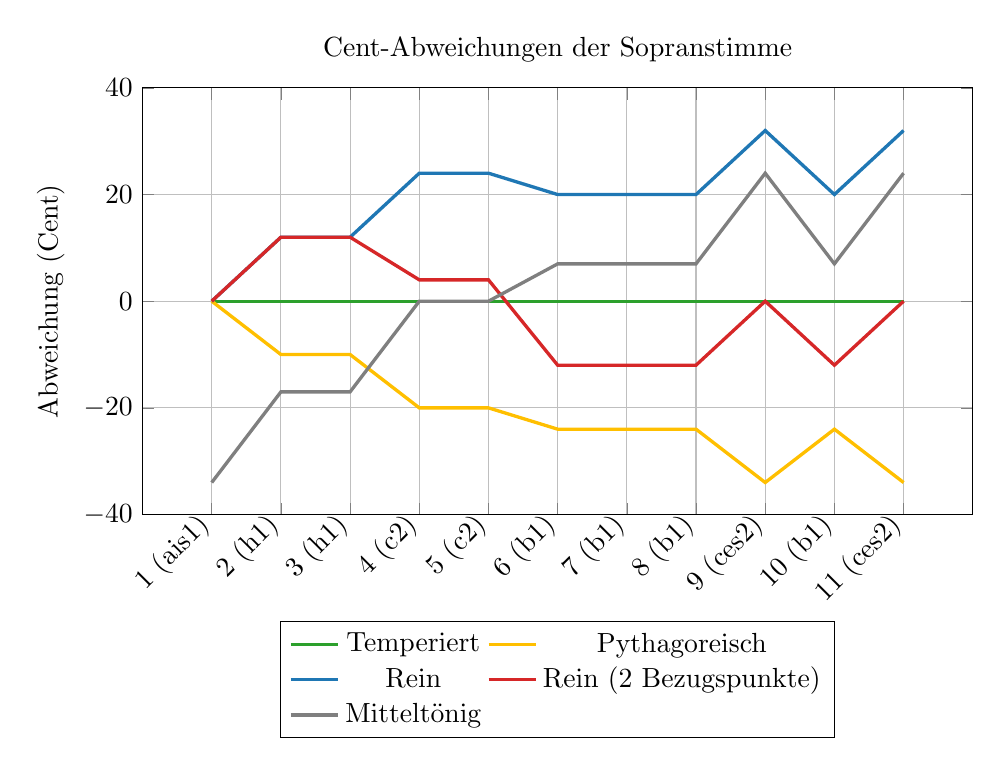
\begin{tikzpicture}
\begin{axis}[
  width=\textwidth,
  height=7cm,
  title={Cent-Abweichungen der Sopranstimme},
  xlabel={},
  ylabel={Abweichung (Cent)},
  ymin=-40, ymax=40,
  xtick={1,...,11},
  xticklabels={
    1 (ais1), 2 (h1), 3 (h1), 4 (c2), 5 (c2), 6 (b1), 7 (b1), 8 (b1), 9 (ces2), 10 (b1), 11 (ces2)
  },
  x tick label style={rotate=45, anchor=east},
  grid=both,
  legend style={at={(0.5,-0.25)}, anchor=north, legend columns=2},
]

% 1) Temperiert (Grün)
\addplot[very thick, color=temperiert] coordinates {
  (1,0) (2,0) (3,0) (4,0) (5,0) (6,0) (7,0) (8,0) (9,0) (10,0) (11,0)
};
\addlegendentry{Temperiert}

% 2) Pythagoreisch (Gelb)
\addplot[very thick, color=pythagoreisch] coordinates {
  (1,0) (2,-10) (3,-10) (4,-20) (5,-20) (6,-24) (7,-24) (8,-24) (9,-34) (10,-24) (11,-34)
};
\addlegendentry{Pythagoreisch}

% 3) Rein (Blau)
\addplot[very thick, color=rein] coordinates {
  (1,0) (2,12) (3,12) (4,24) (5,24) (6,20) (7,20) (8,20) (9,32) (10,20) (11,32)
};
\addlegendentry{Rein}

% 4) Rein (2 Bezugspunkte) (Rot)
\addplot[very thick, color=reinZwei] coordinates {
  (1,0) (2,12) (3,12) (4,4) (5,4) (6,-12) (7,-12) (8,-12) (9,0) (10,-12) (11,0)
};
\addlegendentry{Rein (2 Bezugspunkte)}

% 5) Mitteltönig (Grau)
\addplot[very thick, color=mitteltoenig] coordinates {
  (1,-34) (2,-17) (3,-17) (4,0) (5,0) (6,7) (7,7) (8,7) (9,24) (10,7) (11,24)
};
\addlegendentry{Mitteltönig}

\end{axis}
\end{tikzpicture}%
}
\caption{Cent-Abweichungen der Sopranstimme (f\"unf Presets).}
\end{figure}

\end{document}
